\documentclass[conference]{IEEEtran}
\IEEEoverridecommandlockouts
% The preceding line is only needed to identify funding in the first footnote. If that is unneeded, please comment it out.
% \usepackage{cite}
% Enables Portuguese Brasil
% \usepackage[portuguese]{babel}
%encoding
% Enables code listing
\usepackage{listings}
%--------------------------------------
\usepackage[T1]{fontenc}
\usepackage[utf8]{inputenc}
%--------------------------------------
%Enables the use of greek letter without a math context
\usepackage{textgreek}
%--------------------------------------
%Enables hiperlinks
\usepackage[hidelinks]{hyperref}
%--------------------------------------

\usepackage{amsmath,amssymb,amsfonts}
\usepackage{algorithmic}
\usepackage{graphicx}
\usepackage{textcomp}
\usepackage{xcolor}

% The code style
\usepackage{color}
\definecolor{codegreen}{rgb}{0,0.6,0}
\definecolor{codegray}{rgb}{0.5,0.5,0.5}
\definecolor{codepurple}{rgb}{0.58,0,0.82}
\definecolor{backcolour}{rgb}{0.95,0.95,0.92}

\lstdefinestyle{mystyle}{
	backgroundcolor=\color{backcolour},   
	commentstyle=\color{codegreen},
	keywordstyle=\color{magenta},
	numberstyle=\tiny\color{codegray},
	stringstyle=\color{codepurple},
	basicstyle=\footnotesize,
	breakatwhitespace=false,         
	breaklines=true,                 
	captionpos=b,                    
	keepspaces=true,                 
	numbers=left,                    
	numbersep=2pt,                  
	showspaces=false,                
	showstringspaces=false,
	showtabs=false,                  
	tabsize=2
}
\lstset{style=mystyle}
%---------------------------------------


\def\BibTeX{{\rm B\kern-.05em{\sc i\kern-.025em b}\kern-.08em
    T\kern-.1667em\lower.7ex\hbox{E}\kern-.125emX}}
\begin{document}
\title{Classification of Histopathological Images of Breast Cells between Malignant and Benign Tumors based on Handcrafted Feature Extraction}
\author{Hiago Matheus Brajato \& André Furlan - UNESP - Universidade Estadual Paulista "Júlio de Mesquita Filho"}
\date{2019-11-14}
\maketitle

\begin{abstract}
According to the recent survey published by the International Agency for Research on Cancer (IARC), the breast cancer is one of the most common kinds of cancers diagnosed in the population nowadays. The diagnosis of this type of disease is usually made through the analysis of the breast cells by a specialist after the biopsy and staining, normally made by the combination of hematoxylin and eosin (H \& E). This manual assessment is a time-consuming task and depends on the expertise and perception of the pathologists. In order to overcome this limitations, image processing can be considered as great aid alternative. In this paper is presented an application for the classification of breast cell images between malignant and benign tumors. The developed software includes the principals steps present within the image processing field, such as preprocessing, segmentation, feature extraction and classification, in order to achieve good results in the analysis of a dataset composed by 50 images of malignant and benign tumors.
\end{abstract}

\begin{IEEEkeywords}
Breast Cancer, Image Processing, Diagnosis, Malignant and Benign
\end{IEEEkeywords}

\section{Introduction}
Breast Cancer is a kind of malignant tumor in which cells in the breast grow out of control. In a recent survey called GLOBOCAN \cite{GLOBOCAN} published in 2018 by the IARC, can be visualized the statistics about this type of cancer around the world. The study states that the breast cancer is the second most incident type of cancer in world, with 2 088 049 cases of this disease in the last year, and the number of cases of mortality is equals to 626 679 (about 30\% of total). According to the same study, the breast cancer is the most incident type in Brazil, with 85 620 registered cases in total, and the second most reason of mortalities among the cancers, with 18 842 cases, what represents 22\% of the total cases of breast cancer in Brazil. Figures 1 and 2 in the right graph the information presented until now. In the first chart is possible to visualize the statistics about the world, and in the second one is presented the numbers of cases in Brazil.

\begin{figure}[h]
    \centering
    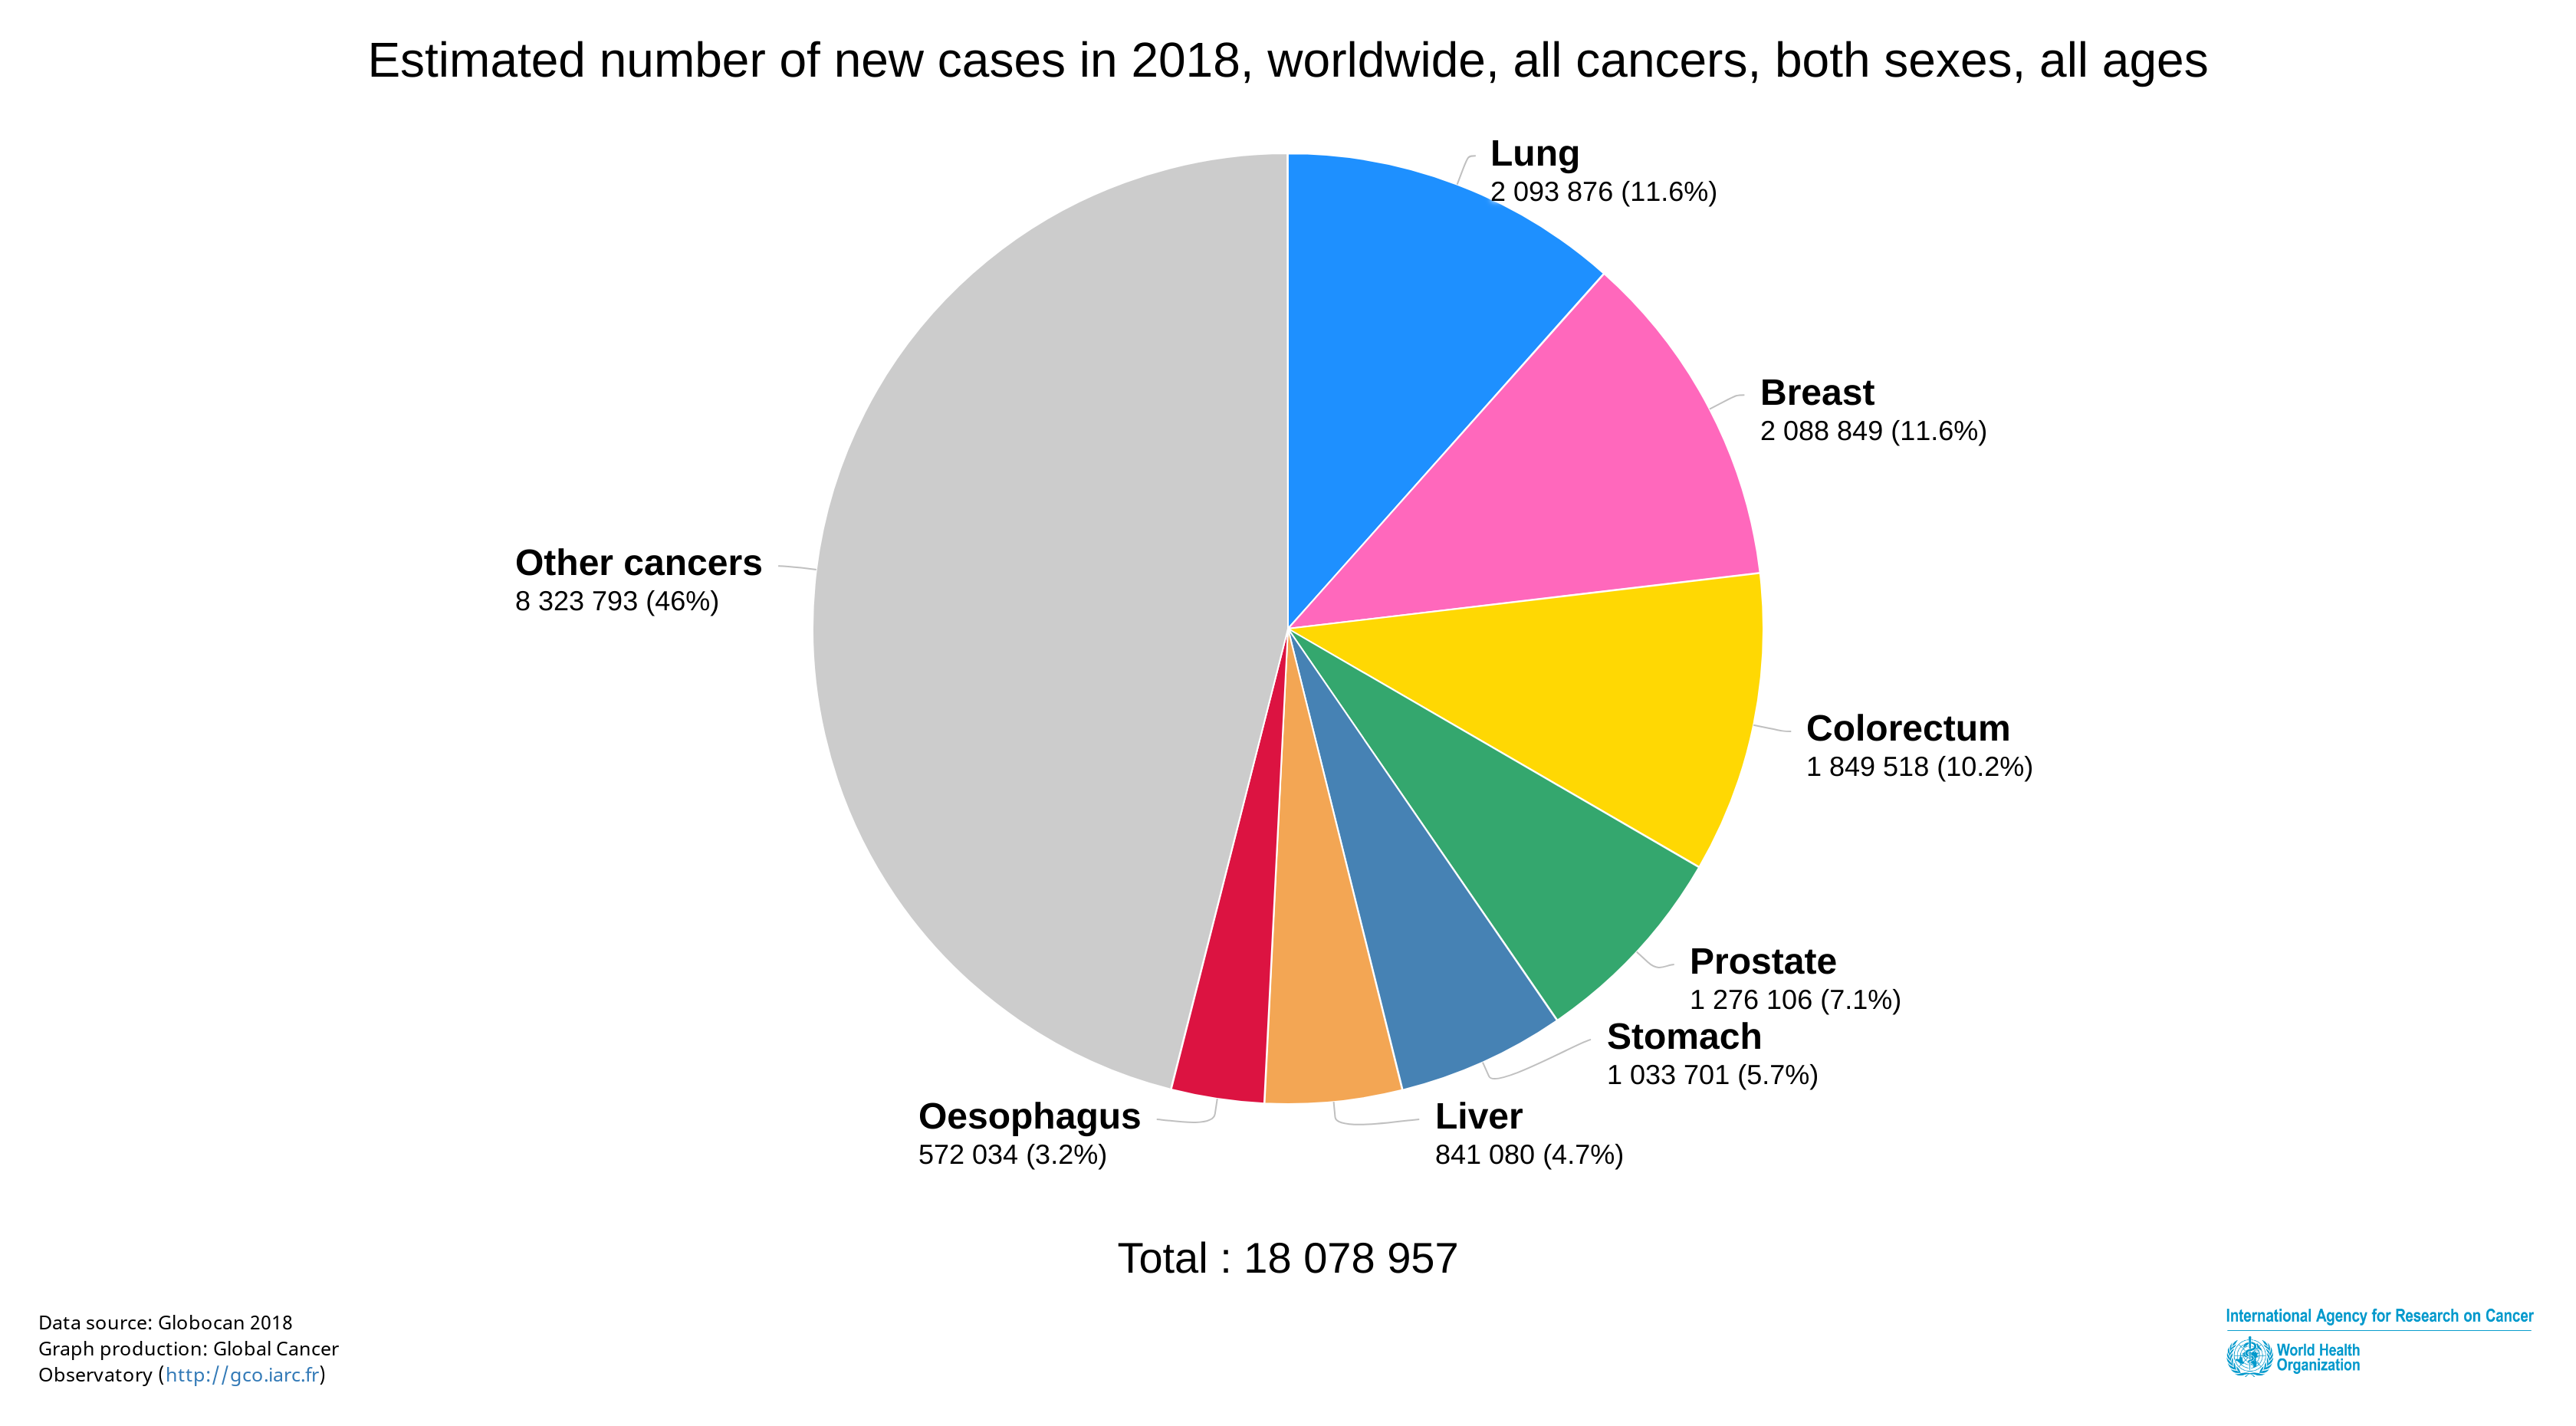
\includegraphics[width=8cm]{images/graphic1.png}
    \caption{Statistics about Incidence of types of Cancer in the World \cite{GLOBOCAN}}
    \label{fig:my_label}
\end{figure}

\begin{figure}[h]
    \centering
    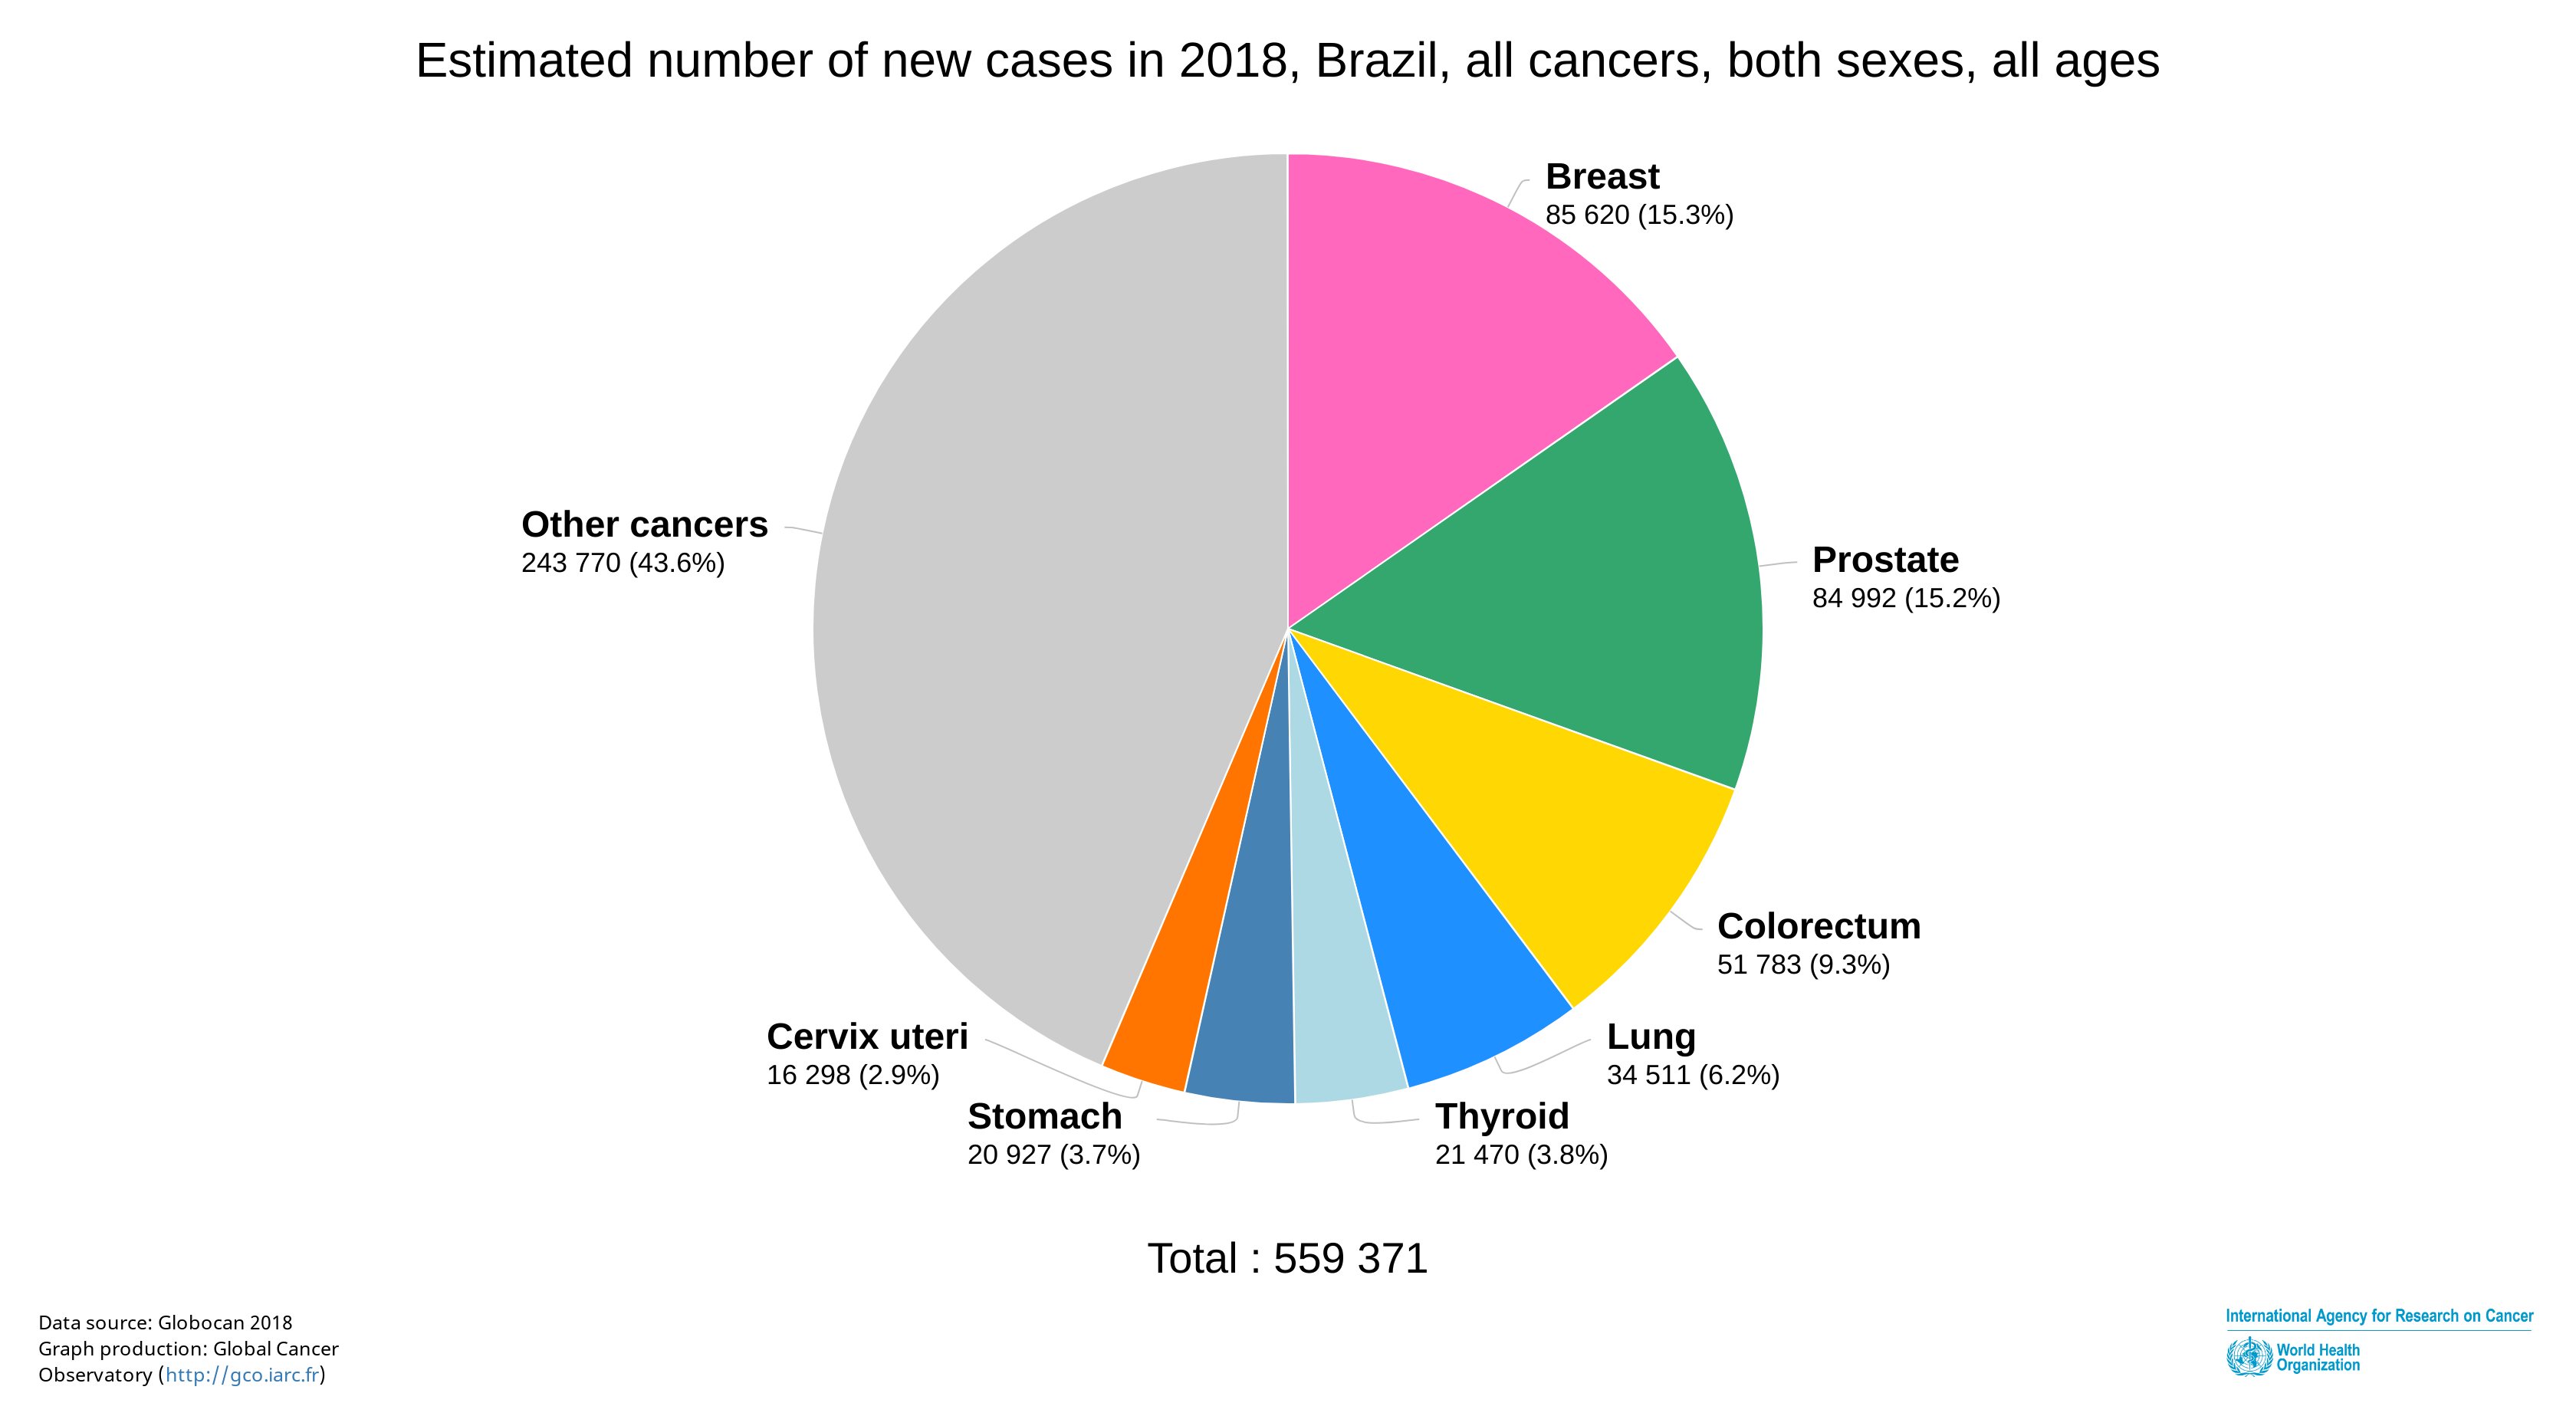
\includegraphics[width=8cm]{images/graphic2.png}
    \caption{Statistics about Incidence of types of Cancer in Brazil \cite{GLOBOCAN}}
    \label{fig:my_label}
\end{figure}

The process of the diagnosis of this type of cancer is usually made by a specialist called pathologist, who is responsible for analysing breast cells acquired through two steps: biopsy and staining. The biopsy step is a test that removes tissues or fluids from the suspicious breast area, and this procedure is the only one that can definitely define if the suspected area is cancerous or not. The staining step is responsible for add color to the cells in order to become easier the visualization of the tissue by the pathologist. After this two steps, the specialized doctor analyses the tissue through a microscope in order to determine if the there are malignant tumors or benign ones. As can be seen, the diagnosis is a really time-consuming task, which depends strongly of the expertise of the specialist. Therefore, is interesting the possibility of having applications that analyse digital images of this breast cells and be able to assist the doctor in the process of diagnosis. \par
The Digital Image Processing is the computational field responsible for dealing with this kind of task, which involves some steps for processing the image in order to achieve the better possible classification rate, in this case between malignant and benign tumors. This paper presents the steps present within of the development of an application responsible for classifying images of breast cells from features extracted, which will be described in the sequence of the paper. Some measures as accuracy, ROC Curve and AUC are compared in order to indicate the best combination of features and classifier. The rest of the paper is organized as follow:  Section II is responsible for presenting the image acquisition, while the section III demonstrates how the filtering of the images was made. Section IV presents the segmentation step, and its impact in the following phases. The step of feature extraction is presented in Section V and the feature selection in Section VI. Finishing the paper, the Section VII presents the process of classification, while Sections VIII and IX present the results and conclusion respectively.

\section{Image Acquisition}
The dataset used in this work is composed by 50 images of breast cells, being that 24 images are of malignant tumors and 26 of benign ones. Informations about this dataset can be found in \cite{artigo_database} and \href{https://bioimage.ucsb.edu/research/bio-segmentation}{\textbf{https://bioimage.ucsb.edu/research/bio-segmentation}}. The Figure 3 below presents a flowchart of the sequence of steps developed in the application.

\begin{figure}[h]
    \centering
    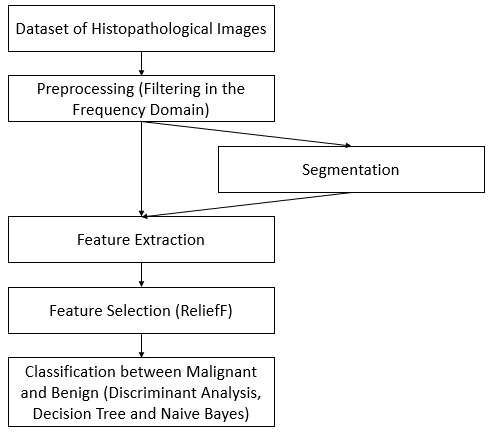
\includegraphics[width=8cm]{images/imagem3.png}
    \caption{Flowchart of the developed method}
    \label{fig:my_label}
\end{figure}

\section{Filtering: Frequency Domain}
The main objective of this section is separate from the noisy background the interesting areas, so the classifiers do not need to evaluate irrelevant data.
The main idea behind it is to subtract the low frequencies components from image and, using morphological operations, remove remaining noises and close the gaps.
\subsection{Filtering}
Two kinds of filters were used:\\
A low pass filter witch is used do highlight the low frequencies features of the image.In this specific case, the radius used was 60 pixels.


\section{Segmentation}
The segmentation is an important step within the image processing, which is responsible for subdividing the an image in regions or objects that compose the signal \cite{Gonzalez:2006:DIP:1076432}, usually, this process is made through the separation of the image between background and object. Several techniques can be used in this process, such as based on thresholding, edge detection, region approaches. In this work, the optimal thresholding technique called Otsu was chosen due to its simplicity and good results. The segmentation was made after the filtering step, and the approach taken in the present work is to subtract the background of the segmented image from the original gray levels image. The code responsible for doing this task and the result produced in the image are shown in the Figure 4.

\begin{figure}[h]
    \centering
    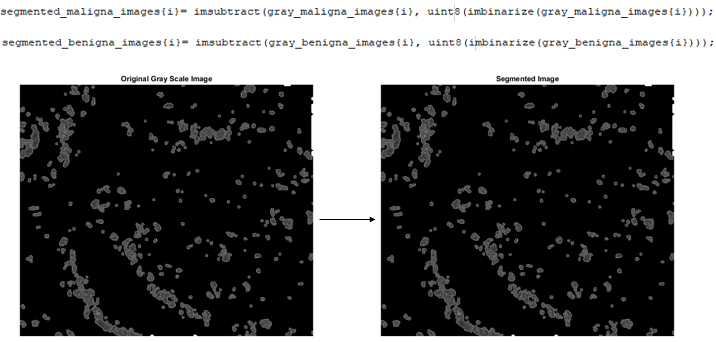
\includegraphics[width=8cm]{images/imagem_segmentacao.png}
    \caption{Segmentation of an Image of Malignant Tumor}
    \label{fig:my_label}
\end{figure}

Although visually is difficult to realize differences between the original image and the segmented one, was checked during the tests that for this image 223 682 pixels were modified in the resulted image in comparison with the original one. Since the dataset is composed for images of resolution 896x768, this quantity of modified pixels achieve around 32\% of the total.\par
Before proceeding for a description of the next steps, it is important to say that the segmentation step is not always necessary in image processing; usually, this step is applied when the following steps as feature extraction and classification are not presenting good results and it is needed to improve the process.\par
Taking this in consideration, in the next sections is presented some measures of classification for segmented and non segmented images, in order to determine the importance and necessity of this step in the whole process.

\section{Feature Extraction}
lorem ipsum, lorem ipsum, lorem ipsum, lorem ipsum, lorem ipsum, lorem ipsum, lorem ipsum, lorem ipsum, lorem ipsum, lorem ipsum, lorem ipsum, 

\section{Feature Selection}
lorem ipsum, lorem ipsum, lorem ipsum, lorem ipsum, lorem ipsum, lorem ipsum, lorem ipsum, lorem ipsum, lorem ipsum, lorem ipsum, lorem ipsum, 

\section{Classification}
lorem ipsum, lorem ipsum, lorem ipsum, lorem ipsum, lorem ipsum, lorem ipsum, lorem ipsum, lorem ipsum, lorem ipsum, lorem ipsum, lorem ipsum, 


\section{Results}
lorem ipsum, lorem ipsum, lorem ipsum, lorem ipsum, lorem ipsum, lorem ipsum, lorem ipsum, lorem ipsum, lorem ipsum, lorem ipsum, lorem ipsum, 

\section{Conclusion}
lorem ipsum, lorem ipsum, lorem ipsum, lorem ipsum, lorem ipsum, lorem ipsum, lorem ipsum, lorem ipsum, lorem ipsum, lorem ipsum, lorem ipsum, 

\bibliographystyle{plain}
\bibliography{references.bib}
\end{document}